%%=====================================================================================
%%
%%       Filename:  Assignment2_Solution.tex
%%
%%    Description:  Solution to problem 2.
%%
%%        Version:  1.0
%%        Created:  02/25/2017
%%       Revision:  none
%%
%%         Author:  Dilawar Singh (), dilawars@ncbs.res.in
%%   Organization:  NCBS Bangalore
%%      Copyright:  Copyright (c) 2017, Dilawar Singh
%%
%%          Notes:  
%%                
%%=====================================================================================

\documentclass[a4paper,10pt]{article}
\usepackage{pgf,tikz}
\usepackage{amsmath}
\usepackage{amssymb}
\usetikzlibrary{shapes,backgrounds,decorations,decorations.pathmorphing}
\usetikzlibrary{calc,positioning}

% Title Page
\title{Solution to Assignment 2} 
\author{Dilawar Singh}
\usepackage{ebgaramond}
\usepackage[T1]{fontenc}
\date{\today}

\begin{document}
\maketitle

Let me start with solutions from assignment submission. 

\section{Drawing without replacement} 

We have a jar with $N$ balls, out of which $b$ are blue and rest are red. I draw
a ball at random but do not put it back.  Clearly it is not a Markovian process
since at each step the probability of drawing red (or blue) ball is changing. At
time zero probability of drawing a blue ball is $\frac{b}{N}$. The probability
of drawing blue ball at next step is either $\frac{b-1}{N-1}$ if drew blue ball
or $\frac{b}{N-1}$ if I drew red ball now. I can define states in the process.
Let say they are {\tt BLUE\_DRAWN} and {\tt RED\_DRAWN}. The transition graph of
this process will look like the following.

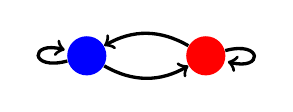
\begin{tikzpicture}[scale=1, every node/.style={circle}, inner sep=5pt ]
    \node[fill=blue] (blue) {};
    \node[fill=red, right=of blue] (red)  {};
    \draw[very thick,->] (blue) to[bend right] (red);
    \draw[very thick,->] (red) to[bend right] (blue);
    \draw[very thick,->] (red) edge[loop right] (red);
    \draw[very thick,->] (blue) edge[loop left] (blue);
    
\end{tikzpicture}    

Where arrow in graph shows the transition to head state given system is in tail
state now. For example, \tikz{ \node[fill=red,circle] (red) {};
\node[fill=blue,circle,right=of red ] (blue) {}; \draw[->] (red) -- node[above]
{$p$} (blue) } depicts the process of drawing blue ball given that red was drawn
just before. The number on arrow $p$ is the probability of this transition. I
leave it upto you to write the transition matrix for this system using these two
states and convince yourself that this is not Markovian.

\paragraph{Converting {\bf this} system to Markovian} The attempt is made by
introducing more states: a {\tt NULL\_BLUE} \tikz \node[circle,fill=blue!50] {};
and {\tt NULL\_RED} \tikz \node[circle,fill=red!50] {}; states. 

The state transition graph is following.

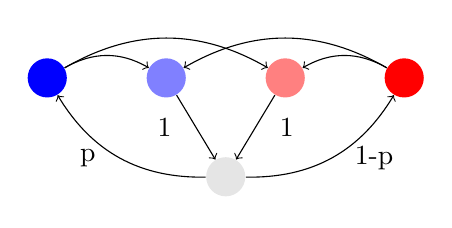
\begin{tikzpicture}[scale=1, every node/.style={circle}, inner sep=5pt ]
    \node[fill=blue] (blue) {};
    \node[fill=blue!50,right=of blue] (nullblue) {};
    \node[fill=red!50, right=of nullblue] (nullred)  {};
    \node[fill=red, right=of nullred] (red)  {};
    \node[fill=black!10,below=of $(nullblue)!0.5!(nullred)$] (null) {};

    \draw[->] (blue) to[bend left] (nullred);
    \draw[->] (blue) to[bend left] (nullblue);

    \draw[->] (red) to[bend right] (nullred);
    \draw[->] (red) to[bend right] (nullblue);

    \draw[->] (nullred) to node[midway,right] {1} (null);
    \draw[->] (nullblue) to node[midway,left] {1} (null);

    \draw[->] (null) to[bend left] node[midway,left] {p} (blue);
    \draw[->] (null) to[bend right] node[midway,right] {1-p} (red);
    
\end{tikzpicture}    

\emph{The state transition graph still does not have constant probabilities. In
short, I could not turn this non-Markovian process to Markovian. However, if
someone has come so far, I've given them credit.
}


\end{document}          

